\chapter*{Proposition 13}
\label{prop:13}

\begin{figure*}[ht]
    \begin{center}
    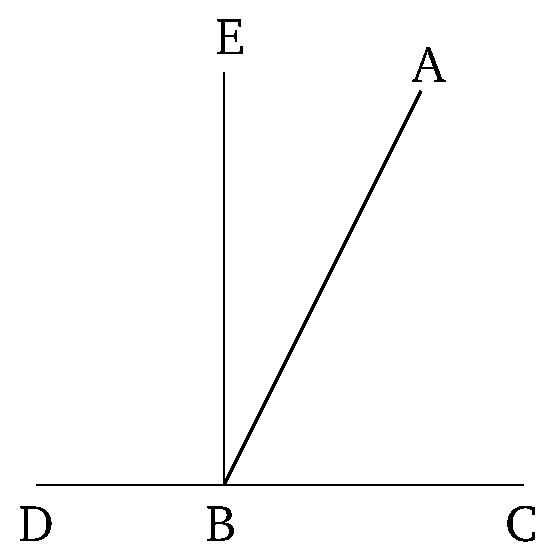
\includegraphics[width=0.5\linewidth]{figures/fig13e.eps}
    \label{fig:prop_13}
    \end{center}
\end{figure*}

If a straight-line stood on a(nother)  straight-line makes angles,
it will certainly either make two right-angles, or (angles whose sum is) equal
to two right-angles. 

For  let some straight-line $AB$ stood on the straight-line $CD$ make the
angles $CBA$ and $ABD$. I say that the angles $CBA$ and $ABD$ are
certainly either two right-angles, or (have a sum) equal to two right-angles.

In fact, if $CBA$ is equal to $ABD$ then they are two right-angles [Def.~\ref{def:10}].
But, if not, let $BE$ have been drawn from the point $B$ at right-angles to [the
straight-line] $CD$ [Prop.~1.11]. Thus, $CBE$ and $EBD$ are two right-angles.
And since $CBE$ is equal to the two (angles) $CBA$ and $ABE$, let $EBD$ have been added
to both. Thus, the (sum of the angles) $CBE$ and $EBD$ is equal to the  (sum of the) three (angles)
$CBA$, $ABE$, and $EBD$ [C.N.~\ref{cn:2}]. Again, since $DBA$ is equal to the two (angles) $DBE$
and $EBA$, let $ABC$ have been added to both. Thus, the (sum of the angles) $DBA$ and $ABC$ is
equal to the (sum of the) three (angles) $DBE$, $EBA$, and $ABC$ [C.N.~\ref{cn:2}]. But (the sum of) $CBE$ and $EBD$ was
also shown (to be) equal to the (sum of the) same three (angles). And things equal to the
same thing are also equal to one another [C.N.~\ref{cn:1}]. Therefore, 
(the sum of) $CBE$ and
$EBD$ is also equal to (the sum of) $DBA$ and $ABC$. But, (the sum of) $CBE$ and $EBD$ is two
right-angles. Thus, (the sum of) $ABD$ and $ABC$ is also equal to two right-angles.

Thus, if a straight-line stood on a(nother)  straight-line makes angles,
it will certainly either make two right-angles, or (angles whose sum is) equal
to two right-angles. (Which is) the very thing it was required to show.



\section*{Commentary}

\begin{proposition}\label{proposition_13}\lean{Elements.Book1.proposition_13}\leanok
    $A$, $B$ are two distinct points on a line $AB$. $C$, $D$ are two distinct points on a different line $CD$. $B$ is between $C$ and $D$. Then, we have $\angle~CBA + \angle~ABD$ is 180 degrees.
\end{proposition}
\begin{proof}
    \uses{proposition_11'}\leanok
    See the original proof by Euclid.
\end{proof}
